%==============================================================================%
% tikz_figures.tex  –  All standalone TikZ visualisations for the dissertation
%
% Each figure is wrapped in \begin{figure}...\end{figure} so it can be
% \input{}–ed from any chapter, or the whole file can be \include{}–d as a
% stand-alone "Figures" appendix.
%==============================================================================%

% ── Helper commands (defined globally so they work inside tikzpicture) ────────
% NTT stage header: #1=x-pos, #2=label, #3=bound
\newcommand{\stagehead}[3]{%
  \node[font=\footnotesize\bfseries\sffamily, align=center] at (#1, 1.35) {#2};%
  \node[font=\scriptsize\ttfamily, align=center, col@darkline]  at (#1, 0.1) {#3};%
}
% NTT group cell: #1=stage-x, #2=group-idx, #3=ydelta(=0.68*g), #4=color
\newcommand{\gcell}[4]{%
  \fill[#4, draw=col@darkline!50, rounded corners=1pt]
    (#1-0.38, -3.45+#3) rectangle (#1+0.38, -3.45+#3+0.58);%
}
% Bounds table row: #1=y, #2=shade(0/1), #3=layer, #4=fwdbounds, #5=invbounds, #6=roundtrip
% Column x: layer=0.0, fwd=2.8, inv=6.5, rt=9.8+0.7=10.5
\newcommand{\bndrow}[6]{%
  \ifthenelse{\equal{#2}{1}}{%
    \fill[col@butterfly!18] (-0.2,#1-0.37) rectangle (11.4,#1+0.37);}{}%
  \node[font=\footnotesize\sffamily, anchor=west]  at (0.0, #1) {#3};%
  \node[font=\scriptsize\ttfamily,   anchor=center, col@highlight]       at (2.8, #1) {#4};%
  \node[font=\scriptsize\ttfamily,   anchor=center, NavyBlue!70!black]   at (6.5, #1) {#5};%
  \node[font=\scriptsize\sffamily\bfseries, anchor=center, OliveGreen!60!black] at (10.5,#1) {#6};%
}

% ── Colour palette ───────────────────────────────────────────────────────────
\colorlet{col@jasmin}   {red!18!white}
\colorlet{col@extract}  {orange!22!white}
\colorlet{col@imperative}{yellow!30!white}
\colorlet{col@algebraic}{green!18!white}
\colorlet{col@endtoend} {cyan!18!white}
\colorlet{col@proof}    {violet!15!white}
\colorlet{col@butterfly}{blue!12!white}
\colorlet{col@arrow}    {black!70}
\colorlet{col@highlight}{BrickRed}
\colorlet{col@darkline} {black!55}

% ── Common TikZ styles ───────────────────────────────────────────────────────
\tikzset{
  layer box/.style = {
    rectangle, draw=col@darkline, rounded corners=4pt,
    minimum width=#1, minimum height=1.15cm,
    align=center, font=\small\sffamily,
    drop shadow={opacity=.12,shadow xshift=1pt,shadow yshift=-1pt},
  },
  layer box/.default = 9cm,
  proof arrow/.style = {
    -Stealth, thick, col@arrow,
  },
  annot/.style = {
    font=\footnotesize\itshape, col@arrow, align=center,
  },
  node wire/.style = {thick, col@arrow},
  butterfly in/.style  = {circle, draw, fill=col@butterfly,
                           minimum size=5pt, inner sep=0pt},
  butterfly out/.style = {circle, draw, fill=col@butterfly!60!black,
                           minimum size=5pt, inner sep=0pt},
}

%==============================================================================%
%  FIGURE 1 — Full Refinement Chain (expanded, annotated)
%==============================================================================%
\begin{figure}[htbp]
\centering
\begin{tikzpicture}[x=1cm, y=1cm, scale=0.88, transform shape]

  %--- Layer boxes -------------------------------------------------------------
  \node[layer box=10.5cm, fill=col@jasmin]
    (L0) at (0, 7.5)
    {\textbf{Layer 0 — Jasmin Source Code}\\[2pt]
     \texttt{poly.jinc}\enspace|\enspace
     \texttt{reduce.jinc}\enspace|\enspace
     \texttt{zetas.jinc}\enspace|\enspace
     \texttt{hpoly.jazz}};

  \node[layer box=10.5cm, fill=col@extract]
    (L1) at (0, 5.4)
    {\textbf{Layer 1 — Extracted EasyCrypt Module}\\[2pt]
     \texttt{Hpoly\_extract.ec}\enspace
     (\texttt{BArray1024.t} operands, machine semantics)};

  \node[layer box=10.5cm, fill=col@imperative]
    (L2) at (0, 3.3)
    {\textbf{Layer 2 — Imperative EasyCrypt Specification}\\[2pt]
     \texttt{NTT\_Fq.ec}\enspace|\enspace
     \texttt{Fq.ec}\enspace|\enspace
     \texttt{Montgomery.ec}
     (\texttt{coeff Array256.t}, loop invariants)};

  \node[layer box=10.5cm, fill=col@algebraic]
    (L3) at (0, 1.2)
    {\textbf{Layer 3 — Abstract Algebraic / Spectral Specification}\\[2pt]
     \texttt{NTTFullSpec.ec}\enspace|\enspace
     \texttt{NTTFullAlgebra.ec}\enspace
     (\(\mathbb{F}_q^{256}\), evaluation formula)};

  %--- Proof step arrows -------------------------------------------------------
  \draw[proof arrow, line width=2pt]
    (L0.south) -- node[right=6pt, annot]
      {\textbf{Step A}\\Jasmin compiler\\extraction\\(machine-checked)}
    (L1.north);

  \draw[proof arrow, line width=2pt]
    (L1.south) -- node[right=6pt, annot]
      {\textbf{Step B}\\pRHL equivalence\\(\texttt{RefJasminNTT.ec})\\word $\leftrightarrow$ int}
    (L2.north);

  \draw[proof arrow, line width=2pt]
    (L2.south) -- node[right=6pt, annot]
      {\textbf{Step C}\\Loop invariant\\induction\\(\texttt{NTTFullAlgebra.ec})}
    (L3.north);

  %--- End-to-end composition --------------------------------------------------
  \node[layer box=4.2cm, fill=col@endtoend, minimum height=2.2cm]
    (E2E) at (-7.5, 4.35)
    {\textbf{End-to-End}\\[3pt]
     \texttt{NTTEndToEnd.ec}\\[3pt]
     \footnotesize
     \texttt{haetae\_jasmin\_ntt}\\
     \texttt{\_correct}\\[2pt]
     $A \circ B \circ C$};

  \draw[proof arrow, dashed, bend left=25]
    (L0.west) to (E2E.north);
  \draw[proof arrow, dashed, bend right=25]
    (L3.west) to (E2E.south);

  %--- Side annotations --------------------------------------------------------
  \node[annot, text=col@darkline, anchor=east] at (-5.7, 7.5)
    {x86-64 assembly\\+ safety proof};
  \node[annot, text=col@darkline, anchor=east] at (-5.7, 5.4)
    {\texttt{W32}/\texttt{W64}\\machine words};
  \node[annot, text=col@darkline, anchor=east] at (-5.7, 3.3)
    {\texttt{int} arithmetic\\16-bit $\to$ 24-bit bounds};
  \node[annot, text=col@darkline, anchor=east] at (-5.7, 1.2)
    {$\hat{f}[i]=\!\!\sum_{j}\!f[j]\,\zeta^{(2\,\mathrm{br}(i)+1)j}$};

\end{tikzpicture}
\caption{Four-layer verification architecture for the \haetae{} NTT.  Solid
         arrows are checked proof steps; dashed arrows show final composition.}
\label{fig:full_arch}
\end{figure}

%==============================================================================%
%  FIGURE 2 — Cooley–Tukey NTT Butterfly (single stage, 8-element example)
%==============================================================================%
\begin{figure}[htbp]
\centering
\begin{tikzpicture}[x=1.5cm, y=0.9cm]

  \def\nleft{4}   % number of element pairs shown

  %--- Input labels (left) ----------------------------------------------------
  \foreach \i/\lab in {
      0/{$a[0]$},
      1/{$a[1]$},
      2/{$a[2]$},
      3/{$a[3]$},
      4/{$a[4]$},
      5/{$a[5]$},
      6/{$a[6]$},
      7/{$a[7]$}}
  {
    \node[anchor=east, font=\small\ttfamily] (in\i) at (0, -\i) {\lab};
  }

  %--- Output labels (right) --------------------------------------------------
  \foreach \i/\lab in {
      0/{$a'[0]$},
      1/{$a'[1]$},
      2/{$a'[2]$},
      3/{$a'[3]$},
      4/{$a'[4]$},
      5/{$a'[5]$},
      6/{$a'[6]$},
      7/{$a'[7]$}}
  {
    \node[anchor=west, font=\small\ttfamily] (out\i) at (4, -\i) {\lab};
  }

  %--- Stage 1 (len=4): butterfly pairs (0,4),(1,5),(2,6),(3,7) ---------------
  \def\sx{1.0}   % x of stage-1 nodes
  \def\ex{2.4}   % x of stage-1 output nodes

  % Butterfly nodes
  \foreach \i in {0,1,2,3} {
    \pgfmathtruncatemacro{\j}{\i+4}
    \node[butterfly in]  (b1up\i)  at (\sx, -\i)  {};
    \node[butterfly out] (b1lo\i)  at (\sx, -\j)  {};
    \node[butterfly in]  (b1oup\i) at (\ex, -\i)  {};
    \node[butterfly out] (b1olo\i) at (\ex, -\j)  {};
  }

  % Straight wires from input
  \foreach \i in {0,1,2,3} {
    \draw[node wire] (in\i) -- (b1up\i);
  }
  \foreach \i in {0,1,2,3} {
    \pgfmathtruncatemacro{\j}{\i+4}
    \draw[node wire] (in\j) -- (b1lo\i);
  }

  % Cross wires (butterfly)
  \foreach \i in {0,1,2,3} {
    \pgfmathtruncatemacro{\j}{\i+4}
    % upper output = upper in + w * lower in
    \draw[node wire, ->, BrickRed!70!black]
      (b1up\i) -- (b1oup\i);
    \draw[node wire, ->, BrickRed!70!black]
      (b1lo\i) to[out=0, in=180] (b1oup\i);
    % lower output = upper in - w * lower in
    \draw[node wire, ->, NavyBlue!70!black]
      (b1up\i) to[out=0, in=180] (b1olo\i);
    \draw[node wire, ->, NavyBlue!70!black]
      (b1lo\i) -- (b1olo\i);
  }

  % Twiddle factor labels
  \foreach \i/\wlab in {0/{$w_0$},1/{$w_1$},2/{$w_2$},3/{$w_3$}} {
    \pgfmathtruncatemacro{\j}{\i+4}
    \node[font=\scriptsize, col@highlight, above=1pt]
      at ($(b1lo\i)!0.5!(b1oup\i)+(0,0.35)$) {\wlab};
  }

  % Output wires
  \foreach \i in {0,1,2,3} {
    \pgfmathtruncatemacro{\j}{\i+4}
    \draw[node wire] (b1oup\i) -- (out\i);
    \draw[node wire] (b1olo\i) -- (out\j);
  }

  %--- Butterfly operation annotation -----------------------------------------
  \node[draw=col@highlight, rounded corners=3pt, fill=col@highlight!8!white,
        align=left, font=\footnotesize, inner sep=6pt]
    (bfann) at (2.0, -8.6)
    {%
      \textbf{Cooley--Tukey butterfly:}\\
      $t \leftarrow w_k \cdot a[j+\ell]$\\
      $a'[j+\ell] \leftarrow a[j] - t$\\
      $a'[j] \leftarrow a[j] + t$\\[3pt]
      {\color{BrickRed!80!black}$\blacksquare$}\ upper path \;
      {\color{NavyBlue!80!black}$\blacksquare$}\ lower path
    };

  %--- Stage label ------------------------------------------------------------
  \node[font=\small\bfseries\sffamily, col@darkline] at (1.7, 0.8)
    {Stage $s$ with $\ell=4$, twiddle counter $k$};

  \draw[decorate, decoration={brace, amplitude=6pt, mirror},
        col@darkline, thick]
    (-0.3, 0.2) -- (-0.3, -3.8)
    node[midway, left=8pt, font=\scriptsize, align=right]
      {upper\\half};
  \draw[decorate, decoration={brace, amplitude=6pt, mirror},
        col@darkline, thick]
    (-0.3, -4.2) -- (-0.3, -7.8)
    node[midway, left=8pt, font=\scriptsize, align=right]
      {lower\\half};

\end{tikzpicture}
\caption{One stage of the Cooley--Tukey butterfly for $n=8$ (shown
         for clarity; the actual NTT uses $n=256$ over 8 stages).
         Red paths carry the $+t$ update to the upper half;
         blue paths carry the $-t$ update to the lower half.
         Each pair of red+blue paths forms one butterfly using twiddle
         factor $w_k = \zeta_0^{\mathrm{brev}_8(k)} \cdot R \bmod q$.}
\label{fig:butterfly}
\end{figure}

%==============================================================================%
%  FIGURE 3 — 8-Stage HAETAE NTT Data Flow (len progression)
%==============================================================================%
\begin{figure}[htbp]
\centering
\begin{tikzpicture}[x=1.75cm, y=0.85cm, scale=0.94, transform shape]
  % Background
  \fill[col@butterfly!28, rounded corners=4pt] (-0.45,-3.6) rectangle (8.45,1.75);
  \draw[col@darkline, dashed] (-0.45,0.40) -- (8.45,0.40);
  \draw[col@darkline, dashed] (-0.45,0.88) -- (8.45,0.88);

  % Stage column headers (hardcoded via \stagehead)
  \stagehead{0}{Input}{16-bit}
  \stagehead{1}{$\ell=128$}{$<\!2^{16}$}
  \stagehead{2}{$\ell=64$} {$<\!2^{17}$}
  \stagehead{3}{$\ell=32$} {$<\!2^{18}$}
  \stagehead{4}{$\ell=16$} {$<\!2^{19}$}
  \stagehead{5}{$\ell=8$}  {$<\!2^{20}$}
  \stagehead{6}{$\ell=4$}  {$<\!2^{21}$}
  \stagehead{7}{$\ell=2$}  {$<\!2^{22}$}
  \stagehead{8}{$\ell=1$}  {23-bit}
  \node[font=\scriptsize\bfseries, text=col@highlight, align=center]
    at (8.00, 1.38) {post\\24-bit};

  % Twiddle counts
  \foreach \s/\cnt in {0/{---},1/{1},2/{2},3/{4},4/{8},5/{16},6/{32},7/{64},8/{128}} {
    \node[font=\scriptsize, col@highlight, align=center] at (\s, 0.65) {$k\mathord{+}$\cnt};
  }

  % Group state grid: 8 groups (g0..g7) × 9 stages
  % A group is "done" (green) at stage s if g < 2^s / 32,
  % i.e., s0: none; s1: g<1=none; s2: g<2; s3: g<4; etc.
  % done(s,g): s=0→0, s=1→g<1, s=2→g<2, s=3→g<4, s=4→g<8 (all)
  % Simplified: done if g <= (2^min(s,3))-2 for s<=3, all for s>=4
  % Group cells: white = pending, green = done
  % s=0..4: all white; s=5: g0 done; s=6: g0,g1; s=7: g0-g3; s=8: all
  \foreach \s in {0,...,4} {
    \foreach \g in {0,...,7} {
      \pgfmathsetmacro{\gyd}{0.68*\g}
      \gcell{\s}{\g}{\gyd}{white}
      \node[font=\tiny\ttfamily, col@darkline!55] at (\s,-3.45+\gyd+0.29) {g\g};
    }
  }
  % s=5
  \pgfmathsetmacro{\gyd}{0.68*0} \gcell{5}{0}{\gyd}{OliveGreen!45}
  \node[font=\tiny\ttfamily,OliveGreen!40!black] at (5,-3.45+\gyd+0.29) {g0};
  \foreach \g in {1,...,7} {
    \pgfmathsetmacro{\gyd}{0.68*\g}
    \gcell{5}{\g}{\gyd}{white}
    \node[font=\tiny\ttfamily, col@darkline!55] at (5,-3.45+\gyd+0.29) {g\g};
  }
  % s=6
  \foreach \g in {0,1} {
    \pgfmathsetmacro{\gyd}{0.68*\g} \gcell{6}{\g}{\gyd}{OliveGreen!45}
    \node[font=\tiny\ttfamily,OliveGreen!40!black] at (6,-3.45+\gyd+0.29) {g\g};
  }
  \foreach \g in {2,...,7} {
    \pgfmathsetmacro{\gyd}{0.68*\g}
    \gcell{6}{\g}{\gyd}{white}
    \node[font=\tiny\ttfamily, col@darkline!55] at (6,-3.45+\gyd+0.29) {g\g};
  }
  % s=7
  \foreach \g in {0,...,3} {
    \pgfmathsetmacro{\gyd}{0.68*\g} \gcell{7}{\g}{\gyd}{OliveGreen!45}
    \node[font=\tiny\ttfamily,OliveGreen!40!black] at (7,-3.45+\gyd+0.29) {g\g};
  }
  \foreach \g in {4,...,7} {
    \pgfmathsetmacro{\gyd}{0.68*\g}
    \gcell{7}{\g}{\gyd}{white}
    \node[font=\tiny\ttfamily, col@darkline!55] at (7,-3.45+\gyd+0.29) {g\g};
  }
  % s=8: all done
  \foreach \g in {0,...,7} {
    \pgfmathsetmacro{\gyd}{0.68*\g} \gcell{8}{\g}{\gyd}{OliveGreen!45}
    \node[font=\tiny\ttfamily,OliveGreen!40!black] at (8,-3.45+\gyd+0.29) {g\g};
  }

  % Stage transition arrows
  \foreach \s in {0,...,7} {
    \pgfmathtruncatemacro{\sn}{\s+1}
    \draw[proof arrow, OliveGreen!70!black, line width=1.4pt]
      (\s+0.41,-1.40) -- (\sn-0.41,-1.40);
    \node[font=\tiny\sffamily, col@darkline] at (\s+0.5,-1.75) {s\sn};
  }

  % Row labels
  \node[font=\scriptsize\bfseries\sffamily, col@darkline] at (-0.02, 1.60) {Stage};
  \node[font=\scriptsize, col@highlight]                  at (-0.02, 0.65) {twiddles};
  \node[font=\scriptsize\ttfamily, col@darkline]          at (-0.02, 0.10) {bound};

  % Legend
  \node[draw=col@darkline!60, rounded corners=3pt, fill=white,
        font=\scriptsize, inner sep=5pt, align=left]
    at (6.80,-2.90)
    {\textcolor{OliveGreen!60!black}{$\blacksquare$} done group\quad
     $\square$ pending};

\end{tikzpicture}
\caption{Data-flow view of the eight-stage forward NTT\@.  Each column
         is one outer-loop iteration ($\ell$ value).  Green cells are groups
         fully processed; white cells are untouched.  The checked coefficient
         invariant starts with a 16-bit input bound and exits with a 24-bit
         postcondition.
         The twiddle counter column ($k{+}$) shows how many twiddle factors
         have been consumed cumulatively.}
\label{fig:ntt_stages}
\end{figure}

%==============================================================================%
%  FIGURE 4 — Montgomery Reduction Dataflow
%==============================================================================%
\begin{figure}[htbp]
\centering
\begin{tikzpicture}[
  box/.style   = {rectangle, draw=col@darkline, rounded corners=3pt,
                  minimum width=2.8cm, minimum height=0.85cm,
                  align=center, font=\small\sffamily,
                  fill=col@imperative},
  op/.style    = {circle, draw=BrickRed!80!black, fill=BrickRed!10,
                  minimum size=0.7cm, font=\small\bfseries},
  wire/.style  = {-Stealth, thick, col@arrow},
  label/.style = {font=\scriptsize, col@darkline},
]

  % Input
  \node[box, minimum width=3.2cm] (inp) at (0, 0) {input $a$ (64-bit)\\$|a| < q \cdot 2^{15}$};

  % Step 1: truncate to 32-bit
  \node[box] (trunc) at (0, -1.9) {truncate $a$\\to 32 bits};
  \draw[wire] (inp.south) -- node[right=3pt, annot]{$(32u)(a)$} (trunc.north);

  % Step 2: multiply by QINV
  \node[op] (mul1) at (2.5, -1.9) {$\times$};
  \node[box, minimum width=2.4cm] (qinv) at (2.5, -0.7) {\texttt{QINV}\\$940508161$};
  \draw[wire] (trunc.east) -- (mul1.west);
  \draw[wire] (qinv.south) -- (mul1.north);

  % Step 3: low 32 bits = m
  \node[box] (m) at (5.0, -1.9) {$m = $ low 32\\of product};
  \draw[wire] (mul1.east) -- node[above=2pt, annot]{mod $2^{32}$} (m.west);

  % Step 4: sign-extend m, multiply by q
  \node[op] (mul2) at (5.0, -3.6) {$\times$};
  \node[box, minimum width=2.0cm] (q_) at (7.2, -3.6) {$q = 64513$};
  \draw[wire] (m.south) -- node[right=3pt, annot]{(64s)} (mul2.north);
  \draw[wire] (q_.west) -- (mul2.east);

  % Step 5: subtract
  \node[op] (sub) at (2.5, -3.6) {$-$};
  \draw[wire] (inp.south|-sub.north) ++(0,0) -- (sub.north)
    node[pos=0, below right=0pt]{};
  \coordinate (apath) at (0, -3.6);
  \draw[wire] (inp.south) -- (apath) -- (sub.west);
  \draw[wire] (mul2.west) -- node[above=2pt, annot]{$m \cdot q$} (sub.east);

  % Step 6: arithmetic right shift
  \node[box] (shift) at (2.5, -5.2) {$\gg_s\, 32$\\(arith shift)};
  \draw[wire] (sub.south) -- node[right=3pt, annot]{$a{-}mq$ (64-bit)} (shift.north);

  % Output
  \node[box, fill=col@algebraic, minimum width=3.2cm]
    (out) at (2.5, -6.9)
    {output $t$ (32-bit)\\$t \equiv a R^{-1} \pmod{q}$\\$|t| < q$};
  \draw[wire] (shift.south) -- node[right=3pt, annot]{divide by $R$} (out.north);

  % Correctness annotation
  \node[draw=OliveGreen!60, fill=OliveGreen!8, rounded corners=3pt,
        font=\scriptsize, inner sep=6pt, align=left]
    at (8.5, -5.5)
    {\textbf{Key invariant:}\\
     $m \cdot q \equiv -a \pmod{2^{32}}$\\
     $\Rightarrow (a - mq) \equiv 0 \pmod{2^{32}}$\\
     $\Rightarrow$ exact integer division\\[3pt]
     $t = \dfrac{a - mq}{R} \equiv aR^{-1}\!\!\pmod{q}$};

  % Title
  \node[font=\small\bfseries\sffamily, col@darkline] at (2.5, 0.7)
    {Signed Montgomery Reduction \texttt{montgomery\_reduce}$(a)$};

\end{tikzpicture}
\caption{Dataflow diagram of the signed Montgomery reduction algorithm.
         The two 32-bit multiplications (\texttt{QINV} and $q$) and the
         arithmetic right shift by 32 are the three core operations.
         The key divisibility invariant ensures that the right shift is
         exact (no remainder), giving the congruence $t \equiv a R^{-1}
         \pmod{q}$.}
\label{fig:montgomery_flow}
\end{figure}

%==============================================================================%
%  FIGURE 5 — Negacyclic Ring and NTT Decomposition
%==============================================================================%
\begin{figure}[htbp]
\centering
\begin{tikzpicture}[x=1cm, y=1cm, scale=0.85, transform shape]

  %--- Ring diagram on the left ------------------------------------------------
  \node[draw=col@darkline, fill=col@imperative!60, rounded corners=6pt,
        minimum width=5.8cm, minimum height=3.6cm, align=center,
        font=\small\sffamily, inner sep=8pt]
    (ring) at (-3.2, 0)
    {\textbf{Polynomial Ring}\\[4pt]
     $R_q = \mathbb{Z}_q[X] / (X^{256}+1)$\\[4pt]
     $q = 64513$,\quad $n = 256$\\[4pt]
     coefficient vector $\in \mathbb{Z}_q^{256}$\\[4pt]
     multiplication = \emph{negacyclic}\\
     convolution};

  %--- Evaluation diagram on the right -----------------------------------------
  \node[draw=col@darkline, fill=col@algebraic!60, rounded corners=6pt,
        minimum width=5.8cm, minimum height=3.6cm, align=center,
        font=\small\sffamily, inner sep=8pt]
    (nttdom) at (3.8, 0)
    {\textbf{NTT Domain}\\[4pt]
     evaluation vector $\in \mathbb{F}_q^{256}$\\[4pt]
     eval.\ points: $\zeta_0^{2\,\mathrm{br}(i)+1}$,\\
     $i=0,\dots,255$\\[4pt]
     multiplication = \emph{pointwise}\\
     $\hat f \odot \hat g$};

  %--- NTT arrow ---------------------------------------------------------------
  \draw[proof arrow, line width=2pt, OliveGreen!70!black]
    (ring.east) to[bend left=18]
    node[above=5pt, font=\small\sffamily\bfseries, OliveGreen!60!black]
      {$\mathsf{NTT}$}
    node[below=5pt, font=\scriptsize, col@darkline]
      {$O(n\log n)$, 8 butterfly stages}
    (nttdom.west);

  \draw[proof arrow, line width=2pt, BrickRed!70!black]
    (nttdom.west) to[bend left=18]
    node[below=5pt, font=\small\sffamily\bfseries, BrickRed!60!black]
      {$\mathsf{INTT}$}
    node[above=5pt, font=\scriptsize, col@darkline]
      {$+$ scaling by $256^{-1}\!\cdot R$}
    (ring.east);

  %--- Isomorphism label -------------------------------------------------------
  \node[font=\small, col@darkline, align=center] at (0.3, 1.5)
    {$\mathsf{NTT} \circ \mathsf{INTT} = \mathrm{id}$};

  %--- CRT decomposition -------------------------------------------------------
  \node[draw=col@darkline, fill=col@butterfly!40, rounded corners=4pt,
        font=\scriptsize\sffamily, inner sep=6pt, align=center]
    (crt) at (0.3, -3.2)
    {\textbf{CRT decomposition:}\enspace
     $R_q \cong \prod_{i=0}^{255} \mathbb{F}_q / (X - \zeta_0^{2\,\mathrm{br}(i)+1})$\\[3pt]
     $X^{256}+1 = \prod_{i=0}^{255}(X - \zeta_0^{2i+1})$ in $\mathbb{F}_q[X]$\\
     (valid since $\zeta_0^{512}=1$, $\zeta_0^{256}=-1$)};

  \draw[col@darkline, dashed, -Stealth] (ring.south) to[bend right=15] (crt.west);
  \draw[col@darkline, dashed, -Stealth] (nttdom.south) to[bend left=15] (crt.east);

  %--- Root circle diagram mini ------------------------------------------------
  \begin{scope}[shift={(0.3, 4.0)}, scale=0.7]
    \draw[col@darkline!50, thick] (0,0) circle (1.3cm);
    \foreach \k in {0,...,7} {
      \pgfmathsetmacro{\ang}{360/8*\k}
      \fill[BrickRed!60] ({1.3*cos(\ang)}, {1.3*sin(\ang)}) circle (2.5pt);
    }
    \node[font=\tiny, col@darkline] at (0,-1.8) {$512$th roots of unity (8 of 256 shown)};
    \draw[-Stealth, col@darkline!50] (-1.6, 0) -- (1.6, 0);
    \draw[-Stealth, col@darkline!50] (0, -1.6) -- (0, 1.6);
    \node[font=\tiny] at (1.45,0.18) {$1$};
    \fill[OliveGreen!80] ({1.3*cos(22.5)},{1.3*sin(22.5)}) circle (3pt);
    \node[font=\tiny, OliveGreen!70!black] at (1.7, 0.55) {$\zeta_0$};
  \end{scope}

\end{tikzpicture}
\caption{The negacyclic polynomial ring $R_q$ and its isomorphism to the NTT
         evaluation domain.  The NTT evaluates the polynomial at all 256
         primitive $512$th roots of unity (red dots on the unit circle).
         This is an instance of the Chinese Remainder Theorem decomposition
         of $R_q$ over $\mathbb{F}_q$.}
\label{fig:ring_ntt}
\end{figure}

%==============================================================================%
%  FIGURE 6 — Bit-Reversal Permutation and Twiddle Index Mapping
%==============================================================================%
\begin{figure}[htbp]
\centering
\begin{tikzpicture}[x=1.15cm, y=0.78cm, scale=0.72, transform shape]

  %--- Title ------------------------------------------------------------------
  \node[font=\small\bfseries\sffamily, col@darkline] at (7.5, 2.1)
    {Bit-reversal $\mathrm{brev}_8 : \{0,\dots,255\}\to\{0,\dots,255\}$
     — first 16 values};

  %--- Grid background (alternating columns) ----------------------------------
  \foreach \k in {0,2,...,14} {
    \fill[col@butterfly!22] (\k-0.45,-0.88) rectangle (\k+0.45,1.68);
  }

  %--- Hardcoded table rows ---------------------------------------------------
  % Row: k value
  \foreach \k/\v in
    {0/0,1/1,2/2,3/3,4/4,5/5,6/6,7/7,
     8/8,9/9,10/10,11/11,12/12,13/13,14/14,15/15}
  { \node[font=\footnotesize\ttfamily] at (\k,1.25) {\v}; }

  % Row: brev_8(k) — hardcoded
  \foreach \k/\v in
    {0/0,1/128,2/64,3/192,4/32,5/160,6/96,7/224,
     8/16,9/144,10/80,11/208,12/48,13/176,14/112,15/240}
  { \node[font=\footnotesize\ttfamily, col@highlight] at (\k,0.42) {\v}; }

  % Row: concrete jzetas[k] values (signed Montgomery form; index 0 is padding)
  \foreach \k/\v in
    {0/0,1/26964,2/-16505,3/22229,4/30746,5/20243,6/19064,7/-31218,
     8/9395,9/-30985,10/22859,11/-8851,12/32144,13/13744,14/21408,15/17599}
  { \node[font=\tiny\ttfamily, col@darkline] at (\k,-0.38) {\v}; }

  %--- Grid lines -------------------------------------------------------------
  \foreach \k in {0,...,16} {
    \draw[col@darkline!30, thin] (\k-0.45,-0.88) -- (\k-0.45,1.68);
  }
  \draw[col@darkline, thick] (-0.45,1.68) -- (15.45,1.68);
  \draw[col@darkline, thick] (-0.45,-0.88) -- (15.45,-0.88);
  \draw[col@darkline]        (-0.45,0.83)  -- (15.45,0.83);
  \draw[col@darkline]        (-0.45,0.02)  -- (15.45,0.02);

  %--- Row labels (left margin) -----------------------------------------------
  \node[font=\footnotesize\bfseries, col@darkline, anchor=east] at (-0.5,1.25)
    {$k$};
  \node[font=\footnotesize\bfseries, col@darkline, anchor=east] at (-0.5,0.42)
    {$\mathrm{brev}_8(k)$};
  \node[font=\footnotesize\bfseries, col@darkline, anchor=east] at (-0.5,-0.38)
    {\texttt{jzetas[k]}};

  %--- Bit-box example (k=3): 00000011 -> 11000000 = 192 ----------------------
  \node[font=\tiny, col@darkline, anchor=east] at (-0.05,-1.55) {$k{=}3$:};

  % k=3 bits b0..b7 = 1,1,0,0,0,0,0,0
  \fill[BrickRed!35,draw=col@darkline,rounded corners=1pt] (0.50,-1.68) rectangle (0.90,-1.35);
  \node[font=\tiny\ttfamily] at (0.70,-1.515) {1};
  \fill[BrickRed!35,draw=col@darkline,rounded corners=1pt] (0.94,-1.68) rectangle (1.34,-1.35);
  \node[font=\tiny\ttfamily] at (1.14,-1.515) {1};
  \fill[white,draw=col@darkline!50,rounded corners=1pt](1.38,-1.68) rectangle (1.78,-1.35);
  \node[font=\tiny\ttfamily] at (1.58,-1.515) {0};
  \fill[white,draw=col@darkline!50,rounded corners=1pt](1.82,-1.68) rectangle (2.22,-1.35);
  \node[font=\tiny\ttfamily] at (2.02,-1.515) {0};
  \fill[white,draw=col@darkline!50,rounded corners=1pt](2.26,-1.68) rectangle (2.66,-1.35);
  \node[font=\tiny\ttfamily] at (2.46,-1.515) {0};
  \fill[white,draw=col@darkline!50,rounded corners=1pt](2.70,-1.68) rectangle (3.10,-1.35);
  \node[font=\tiny\ttfamily] at (2.90,-1.515) {0};
  \fill[white,draw=col@darkline!50,rounded corners=1pt](3.14,-1.68) rectangle (3.54,-1.35);
  \node[font=\tiny\ttfamily] at (3.34,-1.515) {0};
  \fill[white,draw=col@darkline!50,rounded corners=1pt](3.58,-1.68) rectangle (3.98,-1.35);
  \node[font=\tiny\ttfamily] at (3.78,-1.515) {0};

  \node[font=\tiny, col@darkline, anchor=east] at (-0.05,-2.15)
    {\color{BrickRed!75!black}brev:};

  % brev_8(3)=192 bits b0..b7 = 0,0,0,0,0,0,1,1
  \fill[white,draw=col@darkline!50,rounded corners=1pt](0.50,-2.28) rectangle (0.90,-1.95);
  \node[font=\tiny\ttfamily] at (0.70,-2.115) {0};
  \fill[white,draw=col@darkline!50,rounded corners=1pt](0.94,-2.28) rectangle (1.34,-1.95);
  \node[font=\tiny\ttfamily] at (1.14,-2.115) {0};
  \fill[white,draw=col@darkline!50,rounded corners=1pt](1.38,-2.28) rectangle (1.78,-1.95);
  \node[font=\tiny\ttfamily] at (1.58,-2.115) {0};
  \fill[white,draw=col@darkline!50,rounded corners=1pt](1.82,-2.28) rectangle (2.22,-1.95);
  \node[font=\tiny\ttfamily] at (2.02,-2.115) {0};
  \fill[white,draw=col@darkline!50,rounded corners=1pt](2.26,-2.28) rectangle (2.66,-1.95);
  \node[font=\tiny\ttfamily] at (2.46,-2.115) {0};
  \fill[white,draw=col@darkline!50,rounded corners=1pt](2.70,-2.28) rectangle (3.10,-1.95);
  \node[font=\tiny\ttfamily] at (2.90,-2.115) {0};
  \fill[BrickRed!35,draw=col@darkline,rounded corners=1pt](3.14,-2.28) rectangle (3.54,-1.95);
  \node[font=\tiny\ttfamily] at (3.34,-2.115) {1};
  \fill[BrickRed!35,draw=col@darkline,rounded corners=1pt](3.58,-2.28) rectangle (3.98,-1.95);
  \node[font=\tiny\ttfamily] at (3.78,-2.115) {1};

  % Bit position labels b0..b7
  \foreach \b in {0,...,7} {
    \node[font=\tiny, col@darkline!60] at (0.70+\b*0.44,-2.52) {$b_{\b}$};
  }

  % Annotation box
  \node[draw=BrickRed!55, rounded corners=3pt, fill=BrickRed!6,
        font=\scriptsize, inner sep=6pt, align=center]
    (bitann) at (12.5,-1.85)
    {\textbf{Example:}\\
     $k=3 = 00000011_2$\\
     $\mathrm{brev}_8(3) = 11000000_2 = 192$\\[3pt]
     bits: $b_7b_6\cdots b_0 \;\mapsto\; b_0b_1\cdots b_7$};
  \draw[Stealth-, BrickRed!70!black, thick]
    (4.0,-2.0) to[bend right=20] (bitann.west);

\end{tikzpicture}
\caption{The bit-reversal permutation $\mathrm{brev}_8$ for the first 16 table
         values $k = 0,\dots,15$.  Red cells in the bit-pattern boxes highlight
         the set bits.  The bottom row gives the concrete signed
         Montgomery-form table entry \texttt{jzetas[k]}; index 0 is padding,
         and the forward NTT consumes indices 1 through 255.}
\label{fig:brev}
\end{figure}

%==============================================================================%
%  FIGURE 7 — EasyCrypt Proof Structure (Hoare / pRHL judgement stack)
%==============================================================================%
\begin{figure}[htbp]
\centering
\begin{tikzpicture}[x=1cm, y=1cm, scale=0.86, transform shape,
  triple/.style = {
    rectangle, draw=col@darkline, rounded corners=4pt,
    minimum width=12cm, minimum height=1.3cm,
    align=center, font=\small\ttfamily,
    fill=#1, inner sep=6pt,
  },
  hltag/.style = {
    rectangle, draw=col@highlight!70, rounded corners=3pt,
    fill=col@highlight!10, font=\footnotesize\sffamily,
    inner sep=4pt,
  },
]

  %--- Three levels of Hoare judgements ----------------------------------------
  \node[triple=col@jasmin!70]
    (J) at (0, 5.8)
    {%
     \textbf{pRHL equivalence (RefJasminNTT.ec):}\\
     $\texttt{equiv}[\texttt{Hpoly\_extract.M.\_poly\_ntt} \sim
       \texttt{NTT\_Fq.NTT.ntt} :$\\
     $\texttt{poly\_repr\_bound}(\texttt{rp},p,16)
     \;\Longrightarrow\;
     \texttt{poly\_repr\_bound}(\texttt{rp}',p',24)]$};

  \node[triple=col@imperative!70]
    (I) at (0, 3.1)
    {%
     \textbf{Hoare triple (NTT\_Fq.ec):}\\
     $\texttt{hoare}[\texttt{NTT.ntt} :
       \texttt{arg}=(p,\texttt{zetas})$\\
     $\Longrightarrow\;
     \texttt{res} = \texttt{NTT\_loop}(p)]$};

  \node[triple=col@algebraic!70]
    (A) at (0, 0.4)
    {%
     \textbf{Algebraic equality (NTTFullAlgebra.ec):}\\
     $\forall p \in \mathbb{Z}_q^{256}.\;
       \texttt{NTT\_loop}(p) = \texttt{full\_ntt}(p)$\\
     where $\texttt{full\_ntt}(p)[i] =
       \sum_{j=0}^{255} p[j] \cdot \zeta_0^{(2\,\mathrm{brev}_8(i)+1)\cdot j}$};

  \node[triple=col@endtoend, minimum height=1.0cm]
    (E) at (0, -1.8)
    {%
     \textbf{End-to-end (NTTEndToEnd.ec):}\\
     $\texttt{hoare}[\texttt{poly\_ntt\_jazz} :
       \texttt{poly\_repr\_bound}(\texttt{rp},p,16)
       \;\Longrightarrow\;
       \texttt{poly\_repr\_bound}(\texttt{res},\texttt{full\_ntt}(p),24)]$};

  %--- Composition arrows ------------------------------------------------------
  \draw[proof arrow, line width=1.8pt, OliveGreen!70!black]
    (J.south) -- node[right=5pt, annot, OliveGreen!70!black]
      {Step B: apply pRHL $+$ representation} (I.north);

  \draw[proof arrow, line width=1.8pt, OliveGreen!70!black]
    (I.south) -- node[right=5pt, annot, OliveGreen!70!black]
      {Step C: substitute algebraic identity} (A.north);

  \draw[proof arrow, line width=2.2pt, BrickRed!70!black]
    (A.south) -- node[right=5pt, annot, BrickRed!70!black]
      {compose A, B, C} (E.north);

  %--- Side tags ---------------------------------------------------------------
  \node[hltag, anchor=west] at (6.4, 5.8)
    {pRHL};
  \node[hltag, anchor=west] at (6.4, 3.1)
    {HL};
  \node[hltag, anchor=west] at (6.4, 0.4)
    {algebra};
  \node[hltag, anchor=west, fill=BrickRed!12, draw=BrickRed!60]
    at (6.4, -1.8)
    {top-level};

  %--- Proof state tags -------------------------------------------------------
  \node[annot, anchor=east] at (-6.2, 5.8) {machine\\words};
  \node[annot, anchor=east] at (-6.2, 3.1) {field\\arrays};
  \node[annot, anchor=east] at (-6.2, 0.4) {field\\elements};
  \node[annot, anchor=east] at (-6.2,-1.8) {full\\statement};

\end{tikzpicture}
\caption{Structure of the \easycrypt{} proof judgements.  The topmost
         judgement (pRHL) relates machine-word arrays to field-coefficient
         arrays with signed bit-width bounds.  The middle (Hoare) judgement
         captures the loop semantics over field arrays.  The algebraic equality connects the loop output to the
         closed-form spectral sum.  The bottom (end-to-end) judgement
         composes all three.}
\label{fig:ec_proofs}
\end{figure}

%==============================================================================%
%  FIGURE 8 — HAETAE vs. MLKEM NTT Structural Comparison
%==============================================================================%
\begin{figure}[htbp]
\centering
\begin{tikzpicture}[x=1cm, y=1cm, scale=0.60, transform shape,
  scheme/.style = {
    rectangle, draw=col@darkline, rounded corners=6pt,
    minimum width=5.5cm, inner sep=10pt,
    align=left, font=\small\sffamily,
  },
  diff/.style  = {
    fill=BrickRed!12, draw=BrickRed!60, rounded corners=3pt,
    font=\small\sffamily,
  },
  same/.style  = {
    fill=OliveGreen!12, draw=OliveGreen!60, rounded corners=3pt,
    font=\small\sffamily,
  },
]

  %--- HAETAE box --------------------------------------------------------------
  \node[scheme, fill=col@jasmin!50]
    (H) at (-3.2, 0)
    {%
     \textbf{\haetae{} NTT}\\[6pt]
     Modulus $q = 64513$\\
     Degree $n = 256$\\
     Prim.\ root $\zeta_0 = 426$ (512th)\\
     NTT length: \textbf{256-point}\\
     Twiddle exponent: $\mathrm{brev}_8(k)$\\
     Groups / stage: $2^s$, $s=0..7$\\
     Output: fully evaluated\\
     Algebra: $\mathrm{brev}_8$ lemmas\\
     Orthog.\ over 256 roots
    };

  %--- MLKEM box ---------------------------------------------------------------
  \node[scheme, fill=col@algebraic!50]
    (M) at (3.2, 0)
    {%
     \textbf{MLKEM (Kyber) NTT}\\[6pt]
     Modulus $q = 3329$\\
     Degree $n = 256$\\
     Prim.\ root $\zeta_0 = 17$ (256th)\\
     NTT length: \textbf{128-point}\\
     Twiddle exponent: $\mathrm{brev}_7(k)$\\
     Groups / stage: $2^s$, $s=0..6$\\
     Output: incomplete (pairs)\\
     Algebra: $\mathrm{brev}_7$ lemmas\\
     Orthog.\ over 128 roots
    };

  %--- Central "vs" -----------------------------------------------------------
  \node[circle, draw=col@darkline, fill=white,
        minimum size=0.9cm, font=\small\bfseries\sffamily]
    at (0, 0) {vs};

  %--- Difference annotation ---------------------------------------------------
  \node[diff, minimum width=11cm, inner sep=7pt, align=center]
    (diff) at (0, -4.4)
    {\textbf{Key structural difference (invalidates direct algebra reuse):}\\[3pt]
     \haetae{}: twiddle $= \zeta_0^{\mathrm{brev}_8(2^s + g)}$
     \enspace\textbf{(8-bit reversal, full 256-point)}\\
     MLKEM:\enspace twiddle $= \zeta_0^{\mathrm{brev}_7(2g+1)}$
     \enspace\textbf{(7-bit reversal, incomplete 128-point)}};

  \draw[col@darkline, dashed, -Stealth] (H.south) to[bend right=15] (diff.west);
  \draw[col@darkline, dashed, -Stealth] (M.south) to[bend left=15] (diff.east);

  %--- Similarity annotation ---------------------------------------------------
  \node[same, minimum width=11cm, inner sep=7pt, align=center]
    (same) at (0, 3.6)
    {\textbf{Shared aspects (methodology transferable):}
     signed Montgomery REDC,
     Jasmin extraction,
     pRHL refinement pattern,
     coefficient bound tracking};

  \draw[col@darkline, dashed] (H.north) to[bend left=15] (same.west);
  \draw[col@darkline, dashed] (M.north) to[bend right=15] (same.east);

\end{tikzpicture}
\caption{Structural comparison of the \haetae{} and MLKEM NTT\@.
         Green box: aspects where methodology is transferable between
         the two verification projects.  Red box: the critical structural
         difference that prevents direct reuse of MLKEM algebra lemmas.}
\label{fig:haetae_vs_mlkem}
\end{figure}

%==============================================================================%
%  FIGURE 9 — Coefficient Bound Propagation Through All Layers
%==============================================================================%
\begin{figure}[htbp]
\centering
\begin{tikzpicture}[x=0.94cm, y=1cm]

  % Column x positions
  \def\xA{0.0}  % layer name
  \def\xB{2.8}  % forward NTT bound
  \def\xC{6.5}  % inverse NTT bound
  \def\xD{9.8}  % round-trip bound

  %--- Header -----------------------------------------------------------------
  \node[font=\small\bfseries\sffamily, anchor=west] at (\xA, 4.0) {Layer};
  \node[font=\small\bfseries\sffamily, anchor=center] at (\xB, 4.0)
    {Forward NTT bounds};
  \node[font=\small\bfseries\sffamily, anchor=center] at (\xC, 4.0)
    {Inverse NTT bounds};
  \node[font=\small\bfseries\sffamily, anchor=center] at (\xD, 4.0)
    {Identity note};

  \draw[col@darkline, thick] (\xA-0.1, 3.65) -- (\xD+1.5, 3.65);

  %--- Rows (hardcoded 5 rows via global \bndrow) ------------------------------
  \bndrow{3.10}{1}{Jasmin (W32)}%
    {16-bit repr. $\to$ 24-bit repr.}%
    {16-bit repr. $\to$ 16-bit Mont. repr.}%
    {if precondition holds}

  \bndrow{2.25}{0}{Extracted EC}%
    {\texttt{repr\_bound} 16 $\to$ 24}%
    {\texttt{repr\_bound} 16 $\to$ Mont. 16}%
    {\texttt{repr}}

  \bndrow{1.40}{1}{\texttt{NTT\_Fq.ec}}%
    {$p \to \texttt{full\_ntt}(p)$}%
    {$p \to \texttt{full\_invntt}(p)$}%
    {separate maps}

  \bndrow{0.55}{0}{\texttt{NTTFullSpec}}%
    {$p\in\mathbb{Z}_q^{256} \to \hat{p}$}%
    {$\hat{p} \to p$}%
    {math identity}

  \bndrow{-0.30}{1}{\texttt{NTTEndToEnd}}%
    {pre-cond $\to$ post-cond}%
    {pre-cond $\to$ post-cond}%
    {no pipeline lemma}

  %--- Vertical dividers -------------------------------------------------------
  \foreach \x in {2.2, 5.2, 8.8} {
    \draw[col@darkline!40] (\x, 3.65) -- (\x, -1.3);
  }
  \draw[col@darkline, thick] (\xA-0.1, 3.65) -- (\xA-0.1, -1.3);
  \draw[col@darkline, thick] (\xD+1.5, 3.65) -- (\xD+1.5, -1.3);
  \draw[col@darkline, thick] (\xA-0.1, -1.3) -- (\xD+1.5, -1.3);

  %--- Column header rules ----------------------------------------------------
  \draw[col@darkline] (\xA-0.1, 3.65) -- (\xD+1.5, 3.65);

  %--- Annotation --------------------------------------------------------------
  \node[draw=col@darkline, rounded corners=3pt, fill=white,
        font=\scriptsize, inner sep=5pt, align=left]
    at (5.7, -2.4)
    {\textbf{Bit-width summary (forward NTT):}\\[2pt]
     input $16\,\text{bit} \xrightarrow{\text{stage 1}} 17 \xrightarrow{2} 18
       \xrightarrow{3} 19 \xrightarrow{4} 20$\\
     $\xrightarrow{5} 21
       \xrightarrow{6} 22 \xrightarrow{7} 23
       \xrightarrow{\text{post}} 24\,\text{bit}$};

\end{tikzpicture}
\caption{Bound propagation for the checked forward and inverse NTT theorems.}
\label{fig:bounds_table}
\end{figure}

%==============================================================================%
%  FIGURE 10 — EasyCrypt Module/Theory Dependency Graph (detailed)
%==============================================================================%
\begin{figure}[htbp]
\centering
\begin{tikzpicture}[scale=0.90, transform shape,
  x=2.6cm, y=1.6cm,
  ecmod/.style = {
    rectangle, draw=col@darkline, rounded corners=4pt,
    minimum width=2.3cm, minimum height=0.75cm,
    align=center, font=\ttfamily\footnotesize,
    fill=#1,
  },
  ecmod/.default = white,
  depar/.style = {-Stealth, col@arrow, thin},
]

  % Row 0 – foundational theories
  \node[ecmod=col@extract]      (Fq)   at (0,0)   {Fq.ec};
  \node[ecmod=col@extract]      (GFq)  at (1,0)   {GFq.ec};
  \node[ecmod=col@extract]      (FE)   at (2,0)   {Fastexp.ec};
  \node[ecmod=col@extract]      (Arr)  at (3,0)   {Array256.ec};
  \node[ecmod=col@extract]      (Mont) at (4,0)   {Montgomery.ec};

  % Row 1 – ring / word
  \node[ecmod=col@extract!60]   (Rq)   at (1,1)   {Rq.ec};
  \node[ecmod=col@extract!60]   (BA)   at (3,1)   {BArray1024.ec};
  \node[ecmod=col@extract!60]   (WA)   at (4,1)   {WArray1024.ec};

  % Row 2 – extracted and imperative spec
  \node[ecmod=col@imperative!80](Ext)  at (0,2)   {Hpoly\_extract.ec};
  \node[ecmod=col@imperative!80](Nfq)  at (2,2)   {NTT\_Fq.ec};

  % Row 3 – full spec and algebra
  \node[ecmod=col@algebraic!80] (FS)   at (1,3)   {NTTFullSpec.ec};
  \node[ecmod=col@algebraic!80] (FA)   at (3,3)   {NTTFullAlgebra.ec};

  % Row 4 – refinement
  \node[ecmod=col@jasmin!80]    (Ref)  at (2,4)   {RefJasminNTT.ec};

  % Row 5 – end-to-end
  \node[ecmod=col@endtoend, minimum width=3.5cm]
                                (E2E)  at (2,5)   {NTTEndToEnd.ec};

  % Edges
  \draw[depar] (Fq)   -- (Nfq);
  \draw[depar] (GFq)  -- (Nfq);
  \draw[depar] (FE)   -- (Nfq);
  \draw[depar] (Arr)  -- (Nfq);
  \draw[depar] (Mont) -- (Fq);
  \draw[depar] (GFq)  -- (Rq);
  \draw[depar] (Arr)  -- (Rq);
  \draw[depar] (Arr)  -- (BA);
  \draw[depar] (BA)   -- (Ext);
  \draw[depar] (WA)   -- (Ext);
  \draw[depar] (Ext)  -- (Fq);
  \draw[depar] (Rq)   -- (FS);
  \draw[depar] (GFq)  -- (FS);
  \draw[depar] (Arr)  -- (FS);
  \draw[depar] (FS)   -- (FA);
  \draw[depar] (Nfq)  -- (FA);
  \draw[depar] (Fq)   -- (Ref);
  \draw[depar] (Nfq)  -- (Ref);
  \draw[depar] (Ext)  -- (Ref);
  \draw[depar] (Ref)  -- (E2E);
  \draw[depar] (FA)   -- (E2E);
  \draw[depar] (FS)   -- (E2E);
  \draw[depar] (Nfq)  -- (E2E);
  \draw[depar] (Ext)  -- (E2E);

  %--- Legend -----------------------------------------------------------------
  \matrix[draw=col@darkline, rounded corners=3pt, fill=white,
          row sep=3pt, column sep=5pt, inner sep=6pt,
          anchor=north west, font=\scriptsize\sffamily]
    at (4.5, 5.2)
  {
    \node[ecmod=col@extract,    minimum width=1.5cm,minimum height=0.45cm]
      {Foundations}; \\
    \node[ecmod=col@imperative!80, minimum width=1.5cm,minimum height=0.45cm]
      {Imperative}; \\
    \node[ecmod=col@algebraic!80,  minimum width=1.5cm,minimum height=0.45cm]
      {Algebraic}; \\
    \node[ecmod=col@jasmin!80,     minimum width=1.5cm,minimum height=0.45cm]
      {Refinement}; \\
    \node[ecmod=col@endtoend,      minimum width=1.5cm,minimum height=0.45cm]
      {End-to-end}; \\
  };

\end{tikzpicture}
\caption{Detailed \easycrypt{} module dependency graph.  Arrows point from
         dependency to dependent file; standard-library and some transitive
         edges are omitted for readability.  Nodes are colour-coded by layer:
         orange = foundations, yellow = imperative specification,
         green = algebraic specification, red = refinement, cyan = end-to-end.}
\label{fig:dep_graph_full}
\end{figure}
